\section{Methods}
\subsection{Causal Inference}
When studying the relationship between datasets, it is important to distinguish between causation and correlation. While one might find correlations between variables in the data, extra care should be taken before defining causal relationships between the variables. Before making statements on causal relationships, the way the data was generated and any confounders (which may not be captured in the data) must be explored [1]. To ensure that we are not making unsupported claims, we will only seek to find correlation rather than causation in this analysis. 

\subsection{Exploratory Data Analysis}
To analyze the relationship between location and temperature, we first explored the average temperature in the US in the \textit{daily\_global\_weather} dataset for each Latitude and Longitude value. These relationships are shown in Figure~\ref{fig:latlon_temp}. As expected, there is a stronger correlation between Temperature and Latitude than there is between Temperature and Longitude.
\begin{figure}
    \centering
    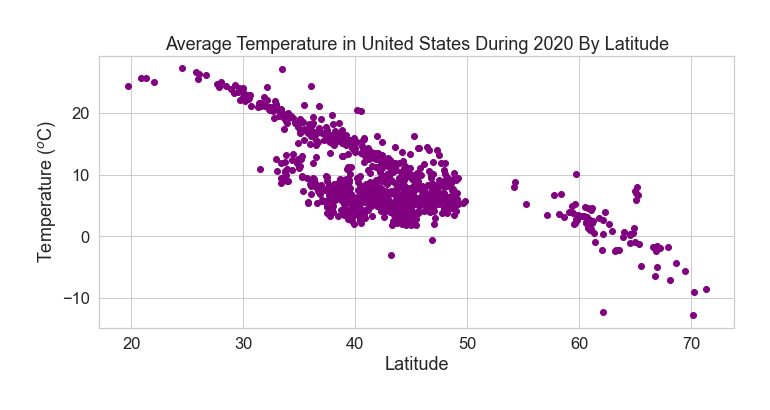
\includegraphics[width=\columnwidth]{figures/USLatTemp.png}
    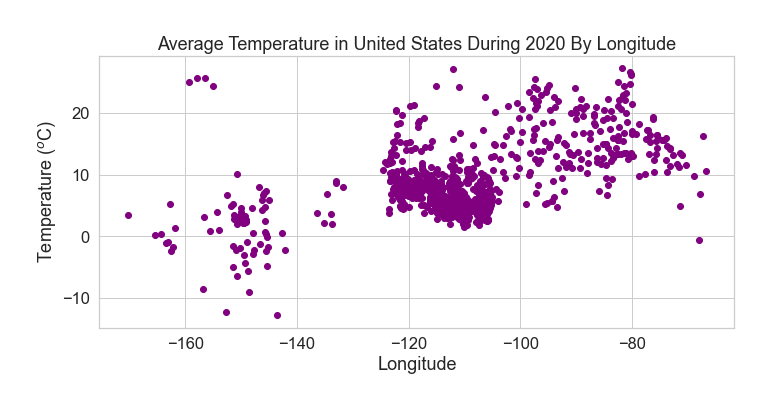
\includegraphics[width=\columnwidth]{figures/USLonTemp.png}
    \caption{Daily Average US Temperature by Latitude (top) and Longitude (bottom).}
    \label{fig:latlon_temp}
\end{figure}


\subsection{Modeling}
Unfortunately I did not have time to fully develop a model. It has been...quite the semester. I will work on this and have something to present in the video on Wednesday. 

We will be including features of Latitude, Longitude, State, Temperature, and CO2 Equivalent Emissions in the model. 